\title{Notes on Organizational Change}
\author{Bil Kleb and Bill Wood}
\date{3 February 2004}

\documentclass{tufte-handout}

 \usepackage{amsmath}  % \text in math mode

 \usepackage{graphicx} % images
   \setkeys{Gin}{width=\linewidth,totalheight=\textheight,keepaspectratio} % defaults
   \graphicspath{{graphics/}} % search path

 \pagestyle{empty} % no page numbers when printing on one sheet, folded in half.

 \AtBeginDocument{ % setup bibliography
	\nobibliography{sample-handout} % bibtex database
	\bibliographystyle{plainnat}    % style
	% Note: you could put these commands at the end of document and
	%       change to \bibliography if you want a "References" section
 }

\begin{document}

\maketitle

\newthought{The Beckhard-Harris-Gleicher} change model\cite{Beckhard1987}
states successful change will happen if and only if the product of the
level of dissatisfaction with status quo, the appeal of the future
vision, and the clarity of the steps necessary to achieve the vision is
greater than the cost of change, measured in terms of emotion, direct
expenses, and lost opportunity.
\begin{displaymath}
  \text{change}
  \,\,\iff\,\,
  \text{dissatisfaction}\times\text{appeal}\times\text{plan}
  \,>\,
  \text{cost}
\end{displaymath}
If any factor is low, the chance for successful change is slim, no matter
how compelling the other factors might appear.
Similarly, if the cost is high, change is not worth pursuing.

\newthought{Satir's model} of well-managed
change\cite{Satir1991}\cite{Weinberg1997}\cite{Beckhard1987}
emphasizes all change entails phases of loss and chaos that, if
unanticipated, will cause a retreat to the original status quo.
A change agent initiates the descent into chaos and then a transforming
idea marks the beginning of the ascent to the new status quo.
\marginnote{Five stage Satir change model diagram \textcopyright\
  stevenmsmith.com.}
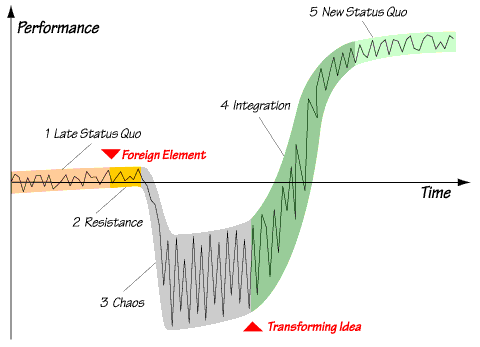
\includegraphics{satir_graph}

\newpage

\newthought{The Bateson Double Bind}\cite{Bateson1956}\cite{Bateson1962}
is a recipe for schizophrenia that should be avoided in organizational
structures:
\begin{compactenum}
 \item Locate a victim who is somehow dependent on you.
 \item Issue a primary injunction with a threat of punishment for
       non-compliance.
 \item Issue a secondary injunction that contradicts the first, again
       coupled with the threat of punishment for non-compliance.
 \item Make the contradiction undiscussible and provide a threat of
       punishment if it is discussed.
 \item Make%
\marginnote{Example: a researcher is dependent upon a mandated support
  service and the support staff imposes a level of service that is
  insufficient.}
       the undiscussibility undiscussible, but make appearances
       that everything is discussible.
 \item Make the victim believe they cannot exit the situation.
\end{compactenum}

\newthought{Block} observes that vision statements are worth something
only to those who make them.\cite{Block1993} 
A vision cannot be handed down from upon high.
Instead, each person or team needs to craft their own vision statement
to have vested ownership and accountability.
One clear requirement, however, is that at each level the vision must be
tied to the one above.

What%
\marginnote{``Simple, clear purpose and principles give rise to complex,
  intelligent behavior,'' says Dee Hock, former CEO of Visa
  International.
  ``Complex rules and regulations give rise to simple, stupid behavior.''}
the core workers do need from those above is a clearly defined,
tangible mission statement that can be used by those at the lowest levels
to make everyday decisions.
NASA's current vision, mission, and goals slides have recently been
cited\cite{Tufte2003}
as embarrassing examples of what not to do:
\vfill
\begin{center}
  
\includegraphics[width=0.5\linewidth]{nasa_vision_sm}
\end{center}
\vfill
\newpage

\newthought{Stop} using PowerPoint bullet list slides for strategic
planning, technical communication, or anything but a marketing pitch.
Lou Gerstner simply shut off the overhead projector when he
began to bring IBM back from the brink of bankruptcy in 1992.
He introduced the novel idea of using complete sentences to describe
how goals would be met.\cite{Gerstner2002}
Furthermore, 3M has documented\cite{Shaw1998}
that bullet lists make us intellectually
lazy in three specific ways: (1)~they are too generic---they offer a
series of things to do that could apply to any business, (2)~they leave
critical relationships unspecified, and (3)~they leave critical
assumptions about how the business works unstated.
Our project planning needs to (a)~embrace change, not try
to suppress it and (b)~use PERT charts with uncertainties
instead of CPM diagrams.\cite{Martin2003}
Budgets are forecast tools, not specifications.
Costs should only be tracked to the same level of precision as benefits
are tracked, because the cost-to-benefit ratio has an approximate
uncertainty equal to the maximum of the cost and benefit
uncertainties.\cite{DeMarco2003}

\end{document}
